\documentclass[10pt, aspectratio=169]{beamer}

% handout
% \documentclass[handout, 10pt]{beamer}

\usepackage{clases}

\title{Investigación Operativa}
\subtitle{Nociones B\'asicas de grafos}
\date{}
\author{Facundo Gutiérrez - Nazareno Faillace Mullen}
\institute{Departamento de Matemática - FCEN - UBA}
% \titlegraphic{\hfill\includegraphics[height=1.5cm]{logo.pdf}}

\begin{document}

\maketitle

\begin{frame}{Repaso de definiciones}
	Un \textit{grafo} est\'a formado por dos conjuntos. $\mathcal{G} = (\mathbb{V,\mathbb{E}}) $. 
	
	Donde $\mathbb{V}$ se denomina el conjunto de \textit{v\'ertices} y $\mathbb{E}$ el conjunto de \textit{aristas}.
	\pause
	\begin{itemize}
		\item $\mathbb{V} = \{1,2,A,B,\star \} $
		\item $\mathbb{E} =  \left \{ \{1,A\},\{1,\star\}, \{2,A\}, \{A,\star\} \right \} $
	\end{itemize}
	
	\begin{center}
		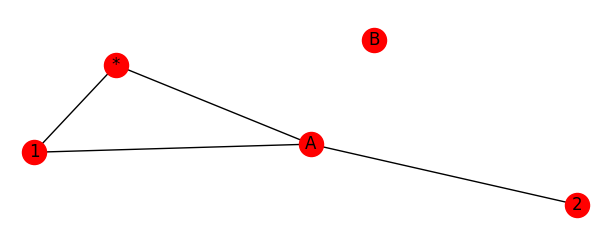
\includegraphics[scale = 0.7]{imagenes/grafo_1.png}
	\end{center}
\end{frame}

\begin{frame}{Repaso de definiciones}
	Un \textit{multigrafo} est\'a formado por dos conjuntos. $\mathcal{G} = (\mathbb{V,\mathbb{E}}) $ 
	
	Donde $\mathbb{V}$ se denomina el conjunto de \textit{v\'ertices} y $\mathbb{E}$ el conjunto de \textit{aristas}. Pero ahora en $\mathbb{E}$ puede haber m\'as de una \textit{arista} que conecte un mismo par de \textit{v\'ertices}.
	\pause
	\begin{itemize}
		\item $\mathbb{V} = \{1,2,A,B,\star \} $
		\item $\mathbb{E} =  \left [ \{1,A\},\{1,\star\}, \{1,\star\}, \{2,A\}, \{A,\star\} \right ] $
	\end{itemize}
	
	\begin{center}
		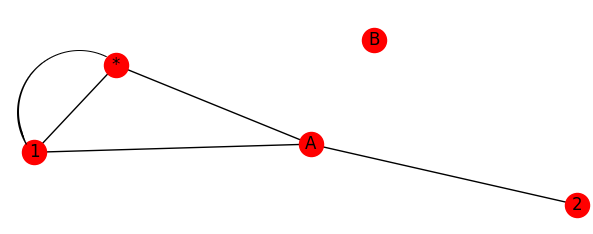
\includegraphics[scale = 0.7]{imagenes/grafo_2.png}
	\end{center}
\end{frame}

\begin{frame}{Repaso de definiciones}
	Un \textit{pseudografo} est\'a formado por dos conjuntos. $\mathcal{G} = (\mathbb{V,\mathbb{E}}) $ 
	
	Donde $\mathbb{V}$ se denomina el conjunto de \textit{v\'ertices} y $\mathbb{E}$ el conjunto de \textit{aristas}. Pero ahora en $\mathbb{E}$ puede haber \textit{aristas} que conecten a un \textit{v\'ertice} con si mismo.
	\pause
	\begin{itemize}
		\item $\mathbb{V} = \{1,2,A,B,\star \} $
		\item $\mathbb{E} =  \left \{ \{1,A\}, \{1,\star\}, \{2,A\}, \{A,\star\}, \{B,B\} \right \} $
	\end{itemize}
	
	\begin{center}
		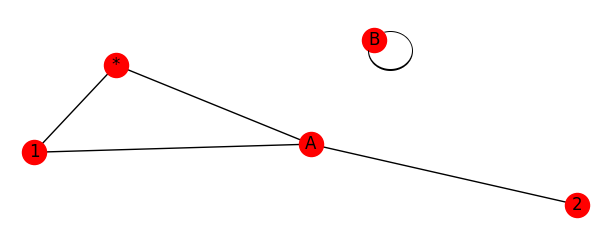
\includegraphics[scale = 0.7]{imagenes/grafo_3.png}
	\end{center}
\end{frame}

\begin{frame}{Repaso de definiciones}
	Dado un v\'ertice $u \in \mathbb{V}$ decimos que un v\'ertice $v$ es \textit{vecino} de $u$ si $\exists e = \{u,v \} \in \mathbb{E}$. A la cantidad de vecinos de $u$ se le llama el \textit{grado} de $u$, y se lo suele notar por $d(u)$.
	\pause  
	
	\begin{itemize}
		\item $\mathcal{N}(A) = \{1,2,\star \} $
		\item $d(A) =  \# \mathcal{N}(A) = \left | \mathcal{N}(A) \right | = 3 $
	\end{itemize}
	
	\begin{center}
		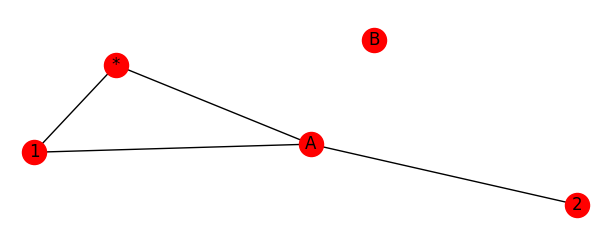
\includegraphics[scale = 0.7]{imagenes/grafo_1.png}
	\end{center}
\end{frame}

\begin{frame}{Repaso de definiciones}
	El \textit{complemento} de un grafo $\mathcal{G} = (\mathbb{V,\mathbb{E}})$, est\'a dado por el grafo $\bar{\mathcal{G}} = (\mathbb{V}',\mathbb{E}')$, donde se tiene una arista por cada par de v\'ertices que no son vecinos en $\mathcal{G}$.
	\pause
	\begin{itemize}
		\item $\mathbb{V}' = \mathbb{V} = \{1,2,A,B,\star \} $
		\item $\mathbb{E}' =  \left \{ \{1,2\},\{1,B\}, \{2,B\}, \{2,\star\}, \{A,B \}, \{B,\star\} \right \} $
	\end{itemize}
	
	\begin{center}
		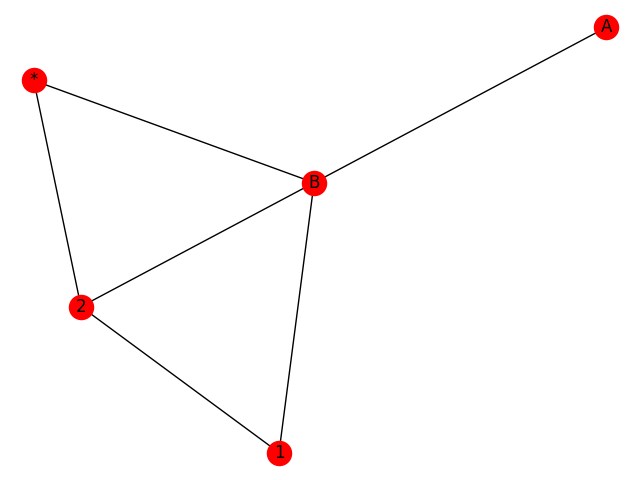
\includegraphics[scale = 0.4]{imagenes/grafo_5.png}
	\end{center}
\end{frame}

\begin{frame}{Repaso de definiciones}
	Dos grafos $\mathcal{G} = (\mathbb{V},\mathbb{E})$ y $\mathcal{H} = (\mathbb{V'},\mathbb{E'})$ se dicen \textit{isomorfos} si existe una funci\'on $f : \mathbb{V} \to \mathbb{V'}$ biyectiva, tal que $e = \{u,v \} \in \mathbb{E} \iff e' = \{f(u),f(v)\} \in \mathbb{E}'$ 
	
	
	\begin{center}
		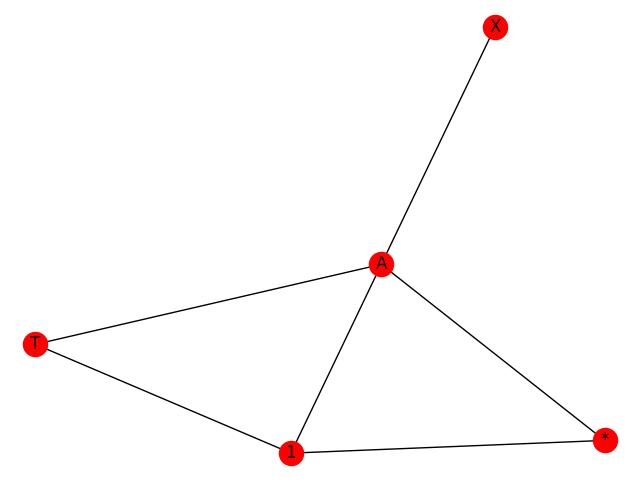
\includegraphics[scale = 0.5]{imagenes/grafo_6.png}
	\end{center}
\end{frame}

\begin{frame}{Repaso de definiciones}
	En un \textit{grafo dirigido} las aristas en $\mathbb{E}$ est\'an dadas por un par ordenado. Ahora cada nodo tiene un vecindario de salida (\textit{out}) y un vecindario de llegada (\textit{in}). En general en grafos dirigidos vamos a utilizar solo el vecindario de salida. 
	\pause
	
	\begin{itemize}
		\item $\mathbb{V} = \{1,2,A,B,\star \} $
		\item $\mathbb{E} =  \left \{ (1,A), (1,\star), (2,A), (A,\star)  \right \} $
		\item $\mathcal{N}_{in}(A) = \{1,2 \} $
		\item $\mathcal{N}_{out}(A) =  \{\star \} $
	\end{itemize}
	
	\begin{center}
		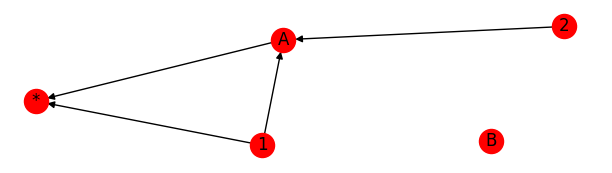
\includegraphics[scale = 0.7]{imagenes/grafo_4.png}
	\end{center}
\end{frame}


\begin{frame}{Propiedad de la suma de los grados}
    \begin{tcolorbox}[title= Propiedad, colback = orange!20, colframe = orange!65!white, coltitle = black]
    Sea $\mathcal{G} = (\mathbb{V},\mathbb{E})$ un grafo, vale la siguiente propiedad:
    $$\displaystyle \sum_{v\in V(G)} d_v = 2|\mathbb{E}|$$
    \end{tcolorbox}
    \footnotesize
    \textbf{Ejercicio:} un grafo tiene 12 aristas y 6 vértices, cada uno de los cuales tiene grado 2 o 5. ¿Cuántos vértices hay de cada grado?
    
    \pause
    \vskip 0.2cm
    
    Sean \textbf{x} la cantidad de nodos de grado 5 e \textbf{y} la cantidad de nodos de grado 2, por el teorema tenemos que:
    $$24 = \displaystyle\sum_{i=1}^6 d_i = 5x+2y  $$
    Por otro lado, como sabemos que el grafo tiene $6$ nodos:
    $$6 = x+y$$
    Entonces se tiene que:
    $$\begin{cases}
    5x+2y = 24\\
    x+y = 6
    \end{cases}
    \Rightarrow x=4 \wedge y=2
    $$ 
	 
\end{frame}

\begin{frame}{Propiedad de la suma de los grados}
\textbf{Ejercicio:} ¿es posible asignar $102$ estudiantes a $35$ computadoras de manera tal que a cada computadora sean asignados $1$ o $3$ estudiantes?
\pause
\vskip 0.35cm
\begin{itemize}
    \itemt Vértices: personas ($V_p$) y computadoras ($V_c$)
    \itemt Aristas:  la arista $(i,j)$, con $i\in V_p,\, j\in V_c$, representa ``el/la estudiante $i$ es asignado/a a la computadora $j$"
\end{itemize}
\pause
\textbf{Obs:} $G$ es un grafo bipartito. \\
\vskip 0.2cm
Por el teorema se tiene que:
$$204=\displaystyle\sum_{v\in V(G)}d_v= \sum_{v\in V_p}d_v + \sum_{v\in V_c}d_v = 102 + \sum_{v\in V_c}d_v $$
\[\Leftrightarrow 102= \sum_{v\in V_c}d_v\]
Como $d_v=1$ o $d_v=3$ para $v\in V_c$, se tiene que $d_v=(2k_v+1)$ para cada $v\in V_c$ siendo $k_v=0$ o $k_v=1$. Luego:
$$102= \sum_{v\in V_c}d_v = \sum_{v\in V_c}(2k_v+1) = 2\sum_{v\in V_c}k_v +35 \Rightarrow 67 = 2\sum_{v\in V_c}k_v \Rightarrow 2\mid67 \quad \text{Abs!}$$
Entonces, no es posible realizar tal asignación.
\end{frame}

\begin{frame}{Lema de apretón de manos}
    \small
    \begin{tcolorbox}[title={Handshaking Lemma (Euler$,$ $1736$)}, colback = orange!20, colframe = orange!65!white, coltitle = black]
    Sea G un grafo finito no dirigido, entonces G tiene un número par de vértices con grado impar 
    \end{tcolorbox}
    \textbf{Demo:} \pause supongamos que G tiene un número impar de vértices con grado impar. Entonces, por la propiedad anterior se tiene que:
    $$\underbrace{2m}_{\text{par}} = \displaystyle\sum_{v\in V(G)} d_v= \underbrace{ \underbrace{\displaystyle\sum_{\substack{v\in V(G)\\ 2 \nmid d_v}}d_v}_{\text{impar}} + \underbrace{\displaystyle\sum_{\substack{v\in V(G)\\ 2 \mid d_v}}d_v}_{\text{par}}}_{\text{impar}} \qquad \text{Abs!}  $$
    El absurdo proviene de suponer que la cantidad de vértices con grado impar es impar. $\blacksquare$
    
\end{frame}


\begin{frame}{Mini ejercicio}

En el \'ultimo torneo universitario de Go se inscribieron 23 participantes. La organizaci\'on del torneo decidi\'o que todos los partidos se lleven a cabo presencialmente en un mismo d\'ia. Por lo tanto, no va a haber tiempo para que jueguen todos contra todos. 


La organizaci\'on del torneo sugiere que cada participante juegue contra exactamente $5$ rivales. ¿Es esto posible? % \pause ¿Y si deciden que cada participante juegue 4 partidos? \pause ¿Y si fueran 24 participantes, podr\'ian jugar 5 partidos cada uno?

\end{frame}

\begin{frame}{Recordando definiciones}
	Dados dos nodos $u,v$, un \textit{camino} de $u$ a $v$ est\'a dado por una secuencia de aristas $e_1, \dots, e_k$ con $e_i = \{a_i,b_i\}$ que satisface:
	\begin{itemize}
		\item $a_1 = u$
		\item $b_k = v$
		\item $b_i = a_{i+1} \forall 1 \leq i \leq k-1$
	\end{itemize}
	
	Adem\'as, la \textit{longitud} de dicho camino est\'a dada por $k$, la cantidad de aristas que lo componen.
	
	Dados dos v\'ertices $u,v$, definimos su $\textit{distancia}$ como la menor longitud de un camino de $u$ a $v$, y la notamos $dist(u,v)$
	
	A la mayor distancia entre dos v\'ertices de un grafo le llamamos el \textit{di\'ametro} del grafo. Es decir: $diam(\mathcal{G}) = \max \{dist(u,v) : u,v \in \mathbb{V} \}$
	\pause	
	
	Decimos que un grafo $\mathcal{G} = (\mathbb{V},\mathbb{E})$ es $\textit{conexo}$ si para todo par de v\'ertices $u,v \in \mathbb{V}$ existe un \textit{camino} que comienza en $u$ y termina en $v$.
\end{frame}

\begin{frame}{Representaci\'on de Grafos}
	Hay muchas formas de representar un grafo. Durante la materia vamos a ver las siguientes:
	\begin{itemize}
		\item Lista de aristas (y cantidad de v\'ertices)
		\item Matriz de adyacencia
		\item Matriz de incidencia
		\item Listas de adyacencia
	\end{itemize}
	
	En la clase de hoy ya vimos la primera durante todos los ejemplos del principio de la clase. ¿Por qu\'e es necesario conocer la cantidad de v\'ertices? 
	\pause
	
	\textbf{Matriz de Adyacencia}: La matriz de adyacencia del grafo $\mathcal{G} = (\mathbb{V},\mathbb{E})$, es la matriz $A \in \{0,1\}^{|\mathbb{V}|\times|\mathbb{V}|}$, que cumple: $[A]_{i,j} = 1 \iff e = \{i,j\} \in \mathbb{E}$.
	
	¿C\'omo es la matriz de adyacencia de un grafo no dirigido? ¿y la de uno dirigido?
	
	
\end{frame}

\begin{frame}{Representaci\'on de Grafos - Matriz de Adyacencia}
	\begin{center}
		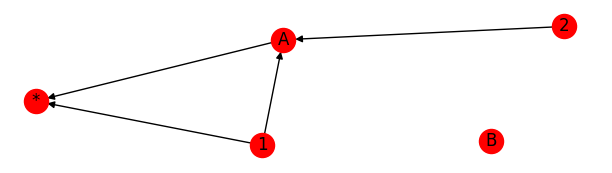
\includegraphics[scale = 0.4]{imagenes/grafo_4.png}
			\pause
			
			\begin{tabular}{|c|c c c c c|} 
				\hline
				        & 1 & 2 & A & B & $\star$ \\ 
				\hline\hline
				1       & 0 & 0 & 1 & 0 & 1 \\ 
				\hline
				2       & 0 & 0 & 1 & 0 & 0 \\
				\hline
				A       & 0 & 0 & 0 & 0 & 1 \\
				\hline
				B       & 0 & 0 & 0 & 0 & 0 \\
				\hline
				$\star$ & 0 & 0 & 0 & 0 & 0 \\  
				\hline
			\end{tabular}
	\end{center}
	\pause
	
	¿C\'omo ser\'ia si las aristas fueran no dirigidas?
\end{frame}

\begin{frame}{Representaci\'on de Grafos - Matriz de Adyacencia}
	\begin{center}
		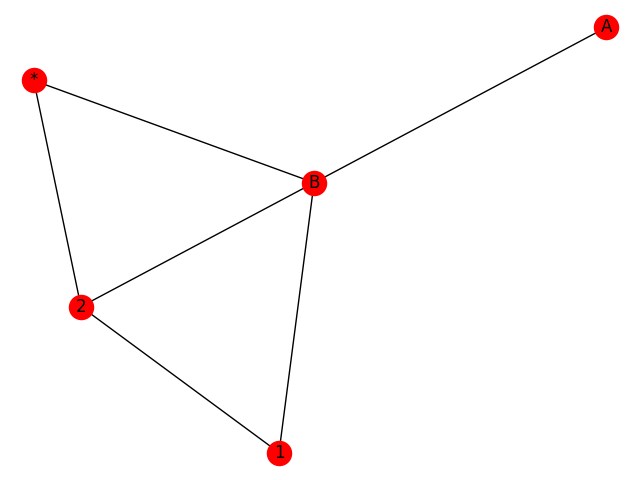
\includegraphics[scale = 0.35]{imagenes/grafo_5.png}
		\pause
		
		\begin{tabular}{|c|c c c c c|} 
			\hline
			        & 1 & 2 & A & B & $\star$ \\ 
			\hline\hline
			1       & 0 & 1 & 0 & 1 & 0 \\ 
			\hline
			2       & 1 & 0 & 0 & 1 & 1 \\
			\hline
			A       & 0 & 0 & 0 & 1 & 0 \\
			\hline
			B       & 1 & 1 & 1 & 0 & 1 \\
			\hline
			$\star$ & 0 & 1 & 0 & 1 & 0 \\  
			\hline
		\end{tabular}
	\end{center}
	
\end{frame}

\begin{frame}{Ejercicio}
	Se tienen $N$ ciudades y $M$ rutas que las conectan. En el plano original es posible llegar de cualquier ciudad a otra mediante combinaciones de rutas.
	
	Las ciudades se dividen en dos grupos. Hay $A$ del grupo 1 y $B$ del grupo 2 (o sea que $A + B = N$). Se quiere renovar el pavimento de algunas rutas de forma tal que de todas las ciudades de grupo 1 se llegue a alguna ciudad de grupo 2 usando solamente rutas con pavimento renovado. ¿Cu\'al es la menor cantidad de rutas que hacen falta pavimentar?
	\pause
	
	Soluci\'on: Clase que viene
\end{frame}

\end{document}

